\chapter{Volumenkontrol}
\label{volumenkontrol}
Formålet med volumenkontrollen er, som beskrevet i afsnit \ref{valg_volumenkontrol}, at gøre det muligt for brugeren at justere volumeniveauet. Dette muliggøres ved to trykknapper, én til op og én til ned. Til at fortælle brugeren hvilket niveau den er indstillet på, skal der være to 7-segmenter, hvor størrelsen af dæmpningen i dB vises. Volumenkontrollen skal have 51 niveauer, så for at lette brugen vælges der, at den skal være i stand til at justere hurtigere, hvis brugeren holder en af de to volumeknapper nede. For at gøre det til en bedre oplevelse skal dette foregå ved en flydende acceleration, fremfor trinvis. Denne funktion skal dog ikke fjerne muligheden for brugeren kan trykke på knapperne med små intervaller og på den måde selv styre justeringshastigheden. \\
De samlede krav til volumenkontrollen er opstillet i tabel \ref{tab:krav_volumenkontrol}.

\begin{table}[h]
\centering
\begin{tabular}{l|r}
\hline\hline
Område & Krav \\
\hline\hline
Frekvensgang & $\pm$ 0,375 dB ved 20 Hz - 20 kHz, ref. 1 kHz \\
& $\pm$ 0,75 dB fra 20 Hz til 63 Hz \\
& $\pm$ 0,75 dB fra 12,5 kHz til 20 kHz \\[4pt]
Dæmpningsområde i & 0 - 50 dB ved 1 kHz \\
volumenkontrol & \\[4pt]
Styring af volumen- & Digital \\
kontrol & \\[4pt]
Antal niveauer i & 51 \\
volumenkontrollen & \\[4pt]
Dæmpning per & 1 dB \\
niveau & \\[4pt]
Input fra brugeren & To trykknapper \\[4pt]
Output til brugeren & To 7-segmenter \\
\hline\hline
\end{tabular}
\caption{Krav til volumenkontrollen}
\label{tab:krav_volumenkontrol}
\end{table}

\clearpage
\section{Design}
\label{volumenkontrol-design}
For at give et overblik er der lavet et blokdiagram der beskriver hvordan volumenkontrollen skal fungere, det er vist på figur \ref{fig:blokdiagram_volumenkontrol}.

\begin{figure}[h]
\centering
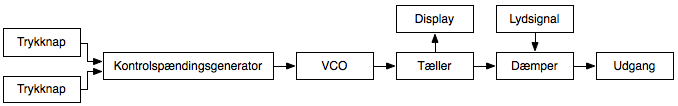
\includegraphics[scale=0.5]{teknisk/volumenkontrol/blokdiagram-volumenkontrol.png}
\caption{Overordnet blokdiagram over volumenkontrollen}
\label{fig:blokdiagram_volumenkontrol}
\end{figure}

For at opnå en accelererende justering i volumenkontrollen, benyttes en Voltage Controlled Oscillator, VCO, med varierende kontrolsignal. VCO'ens signal vil således have en lineært stigende frekvens, for et lineært stigende kontrolsignal. Dette kontrolsignal genereres ved at oplade spændingen over en kondensator med en konstant strøm, fra en konstantstrømsgenerator. VCO'ens signal skal også kunne tvinges tilbage til udgangspunktet, frekvensmæssigt, hvilket klares ved at aflade kontrolsignalt over samme kondensator. Denne afladning opnåes gennem en transistor, som styres udfra brugerens tryk på volumenkontrollens to trykknapper. VCO'ens udgangssignal bruges som clocksignal til en tæller, som kan tælle fra 0 til 50. Udgangssignalet af denne tæller bruges til to ting. For det første bruges signalet i en efterfølgende dæmper, hvor lydsignalet dæmpes mellem 0 og 50 dB, alt efter værdien tælleren står på. For det andet bruges tællerens udgangssignal til at vise størrelsen af dæmpningen i et display bestående af to 7-segmenter.
Det elektriske diagram, som er vist på figur \ref{fig:volumenkontrol_diagram}, indeholder flere blokke, da der under designet af volumenkontrollen tages flere hensyn, som ikke er beskrevet i det ovenstående. Figur \ref{fig:volumenkontrol_diagram} viser desuden kun hvad der på figur \ref{fig:blokdiagram_volumenkontrol} svarer til blokkene til og med signalet ind i tælleren. De elektriske diagrammer for resten af blokkene vises under hver enkelt beskrivelse i den resterende del af dette afsnit.
%For at have en accelererende volumenkontrol benyttes en VCO. VCO'en skal således have en stigende frekvens, det gøres ved at kontrolsignalet er stigende. Det lineært stigende signal laves ved at oplade en ladekondensator med en konstant strøm. Den konstante strøm generes af en konstantstrømsgenerator. Der skal også være mulighed for at nulstille VCO'en, dette gøres ved at aflade ladekondensatoren gennem en transistor der styres af volumenknapperne gennem en AND-gate. AND-gaten bruges for at sikre ladekondensatoren aflades ved både volumen op og ned. Hvis brugeren blot trykker kort én gang på en af volumenknapperne skal der ikke tælles, dette sikres ved at forsinke VCO'ens kontrolsignal. For at undgå forkert opførsels benyttes en XOR-gate til at sikre at volumenknapperne ikke er ens, resultatet af denne operation kobles sammen med VCO'en output gennem en AND-gate, for at sikre der ikke ændres på volumen medmindre brugeren trykker på volumenknapperne. Resultatet af denne AND-gate bruges som CLK-signal til en op/ned tæller, der også informere om retningen af volumen ned knappen. Tællerens output bruges både til at vise den aktuelle volumen indstilling på et display og til at styre en dæmper der dæmper lydsignalet. Blokdiagrammet er afbilledet på figur \ref{fig:volumenkontrol_opbygning}.\\ På figur \ref{fig:volumenkontrol_diagram} er vist det elektriske diagram for volumenkontrollen.\\ Der er kun vist blokkene til og med den anden AND-gate, resten af diagrammet er vist under de enkelte afsnit.

\begin{figure}[h]
\centering
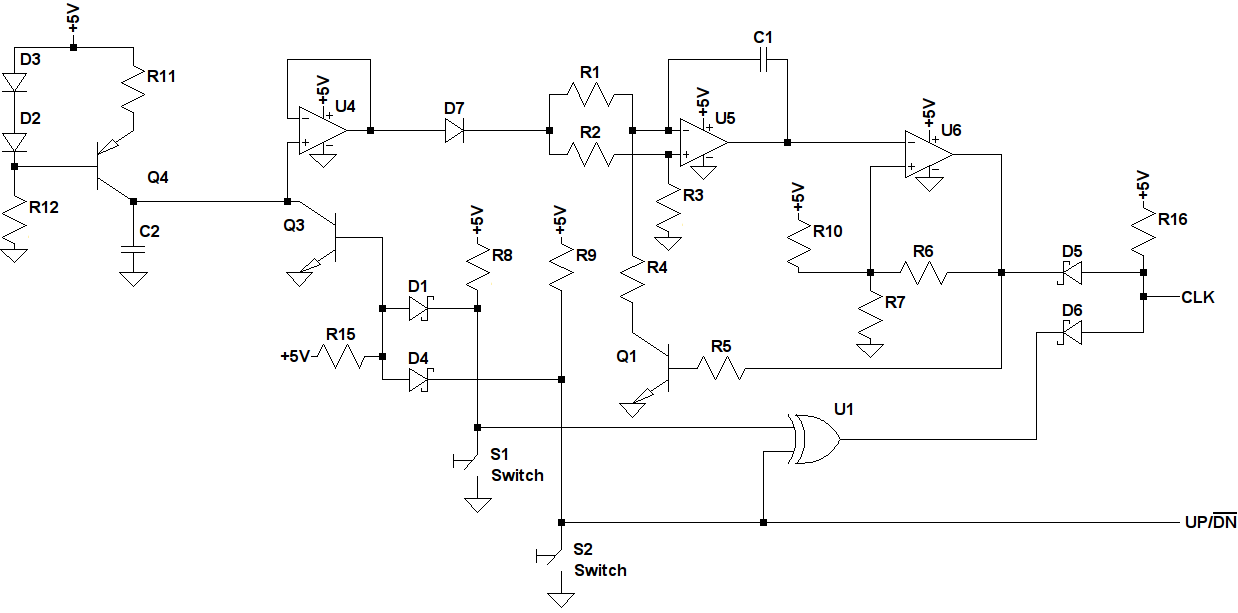
\includegraphics[width=\textwidth]{teknisk/volumenkontrol/diagram-med-kasser.png}
\caption{Elektrisk diagram over volumenkontrollen}
\label{fig:volumenkontrol_diagram}
\end{figure}

\subsection*{Konstantstrømsgenerator}
\label{volumenkontrol-design-konstantstroemsgenerator}

Konstantstrømsgeneratorens opgave er at levere en konstant strøm, denne strøm bruges til at oplade en kondensator (ladekondensatoren). Når en kondensator lades med en konstant strøm, vil spændingen over den stige lineært, dette fremgår også af ligning (\ref{equ:konstantstroemsgenerator1}).

\begin{equation}
\label{equ:konstantstroemsgenerator1}
V = \frac{I \cdot t}{C}
\end{equation}

Konstantstrømsgeneratoren er designet med udgangspunkt i at der vil være et spændingsfald på 0,5 V over $D_2$, $D_3$, $R_{11}$ og $Q_{4_{BE}}$. I databladet for 1N4148 \cite{1n4148-datablad} fremgår det at den vil have en spændingen, $V_D$, over sig på 0,5 V ved en strøm, $I_F$, på 0,1 mA. Strømmen igennem dioderne er givet ved den strøm, der vil løbe igennem det der kommer efter dem, i dette tilfælde modstanden $R_{12}$. Størrelsen af $R_{12}$ er således givet ved ligning (\ref{equ:konstantstroemsgenerator2}).

\begin{equation}
\label{equ:konstantstroemsgenerator2}
R_{12} = \frac{V_{CC} - 2 \cdot V_D}{I_F} = \mathrm{\frac{5~V - 2 \cdot 0,5~V}{0,1~mA} = 40~k\ohm}
\end{equation}

Da der nu ligger en konstant spænding over begge dioder, kan man opfatte dioden i transistoren som siddende parallelt med $D_2$ og $D_3$ og dermed have det samme spændingsfald som $D_2$. Dette giver, at der findes det samme, konstante, spændingsfald over $R_{11}$ som over $D_3$, hvilket giver en konstant strøm gennem $R_{11}$.
Kondensatoren, $C_2$, kaldes ladekondensatoren og den har en kapacitet på 5 $\mu$F.  Den oplades fra 0 V til $V_{CC} - V_D - V_{\mathrm{CEsat}}$ = 4,4 V, hvor $V_D$ er spændingen over én diode og $V_{\mathrm{CEsat}}$ er collector-emitter saturationspændingen på 0,1 V. Opladetiden er desuden valgt til at skulle være 3 sekunder. Udfra disse to ting kan den konstante strøm, $I_{\mathrm{const}}$, nu beregnes ved udregningen i formel (\ref{equ:konstantstroemsgenerator3}).

\begin{equation}
\label{equ:konstantstroemsgenerator3}
V_{CC} - V_D - V_{\mathrm{CEsat}} = \frac{I_{\mathrm{const}} \cdot t}{C_2} \Rightarrow \mathrm{4,4~V} = \frac{I_{\mathrm{const}} \cdot 3~\mathrm{s}}{5~\mu \mathrm{F}} \Rightarrow I_{\mathrm{const}} = \mathrm{7,3~\mu A}
\end{equation}

Spændingen over $R_{11}$ er, som tidligere nævnt, 0,5 V og strømmen igennem den er altså 7,3$\mu$A. Modstanden $R_11$ kan dermed beregnes ved Ohms lov, som vist i udregningen i formel (\ref{equ:konstantstroemsgenerator4}).

\begin{equation}
\label{equ:konstantstroemsgenerator4}
V_D = R_{11} \cdot I_{\mathrm{const}} \Rightarrow \mathrm{0,5~V} = R_{11} \cdot \mathrm{7,3~\mu A} \Rightarrow R_{11} = \mathrm{68,2~k\ohm}
\end{equation}

\subsection*{Starter}
\label{volumenkontrol-design-starter}

Starterens opgave er at holde spændingen over ladekondensatoren på 0 V, når der ikke trykkes på en af volumenknapperne. Dette gøres ved at lede al den strøm som konstantstrømsgeneratoren leverer til stel. Så snart der trykkes på en af volumenknapperne, vil basis på transistoren blive trukket lav, hvilket vil afbryde collector-emitter strømmen. Dette gøres for at sikre at ladekondensatoren er klar til at starte opladningen med det samme.
\subsection*{Buffer med forsinkelse}
\label{volumenkontrol-design-buffer}

Bufferen sikrer at ladekondensatoren bliver lineært opladet ved at sørge for at belastning på konstantstrømsgeneratoren og ladekondensatoren undgåes. Forsinkelsen laves ved hjælp af en diode, da spændingen over den minimum skal vokse til en diodespænding, før der kommer en kontrolspænding til VCO'en. Forsinkningen er derfor direkte afhængig af diodespændingen, hvilket betyder, at der for at kunne indstille på forsinkelsesperioden skal indsættes en anden diode, med en anden $V_{D}$.